% Build from report/:  pdflatex report.tex && pdflatex report.tex && cp report.pdf ../report.pdf
% Tables in tex/ and figures in figures/report/ are generated from tables/ by
% make_report_tables.py and make_report_figures.py.
\documentclass[11pt,a4paper]{article}
\usepackage[a4paper,margin=1.8cm]{geometry}
\usepackage{lmodern}% loaded before fontenc: this TeX lacks the cm-super (ecrm) metrics
\usepackage[T1]{fontenc}
\usepackage{amsmath}
\usepackage{graphicx}
\usepackage{booktabs}
\usepackage{array}
\usepackage[font=small,labelfont=bf,skip=3pt]{caption}
\usepackage{enumitem}
\usepackage{titlesec}
\usepackage[hidelinks]{hyperref}

\titlespacing*{\section}{0pt}{7pt}{3pt}
\titlespacing*{\subsection}{0pt}{5pt}{2pt}
\titleformat*{\subsection}{\normalsize\bfseries}
\setlist{nosep,leftmargin=1.2em}
\setlength{\parskip}{2pt}
\setlength{\textfloatsep}{8pt}
\setlength{\floatsep}{6pt}
\setlength{\intextsep}{6pt}
\renewcommand{\arraystretch}{1.05}
\makeatletter\newcommand{\rows}[1]{\@@input #1 }\makeatother % \input is not expandable inside tabular
\newcommand{\hf}[1]{\href{https://huggingface.co/Devatri/anlp-assignment2-#1}{\texttt{Devatri/anlp-assignment2-#1}}}

\title{\vspace{-1.6cm}\textbf{Advanced NLP --- Assignment 2}\\[2pt]
\large Mixture-of-Experts Translation, Optimizers Written from Scratch, and Decoding Strategies}
\author{\textit{[Divyansh Atri]} \quad \textit{[2024113001]}}
\date{\vspace{-0.55cm}October 2026}

\begin{document}
\maketitle
\vspace{-0.4cm}

\noindent This report covers the three tasks of the assignment. \textbf{Part~1} compares five feed-forward (FFN) designs, one dense and four Mixture-of-Experts (MoE), inside a Transformer that translates Vietnamese and Japanese into English. \textbf{Part~2} implements AdamW, NAdamW, Lion, Muon and (bonus) Sophia by hand and compares them on one language model. \textbf{Part~3} implements greedy, beam, top-$k$, top-$p$ and pure sampling decoding on the forward pass of a pretrained Pythia-160M and evaluates them on ROCStories. All jobs ran on the IIIT ADA cluster with one NVIDIA RTX 2080 Ti (11\,GB) each. Every number below comes from the result files written by these runs. The trained checkpoints are public on Hugging Face:

\begin{center}\footnotesize
\begin{tabular}{@{}ll@{\hspace{1.2em}}ll@{}}
\toprule
\multicolumn{2}{@{}l}{\textbf{Part 1} (checkpoint, tokenizer, code, full-test BLEU)} & \multicolumn{2}{l@{}}{\textbf{Part 2} (checkpoint, config, metrics, generations, \texttt{model.py})}\\
\midrule
M1 dense & \hf{part1-model1} & AdamW & \hf{part2-adamw}\\
M2 & \hf{part1-model2} & NAdamW & \hf{part2-nadamw}\\
M3 & \hf{part1-model3} & Lion & \hf{part2-lion}\\
M4 & \hf{part1-model4} & Muon & \hf{part2-muon}\\
M5 & \hf{part1-model5} & Sophia & \hf{part2-sophia}\\
\bottomrule
\end{tabular}
\end{center}

%======================================================================
\section{Part 1: Mixture-of-Experts FFN variants}

\subsection{Setup}
\textbf{Data.} \texttt{belumind/en-vi-ja-curated-500k-triplets} (pinned revision) provides (vi, ja, en) triplets with official train/validation/test splits. After NFC normalisation, removal of training rows whose English target also occurs in validation or test, and removal of over-length examples (nothing is truncated; a triplet is dropped if either direction is too long), 446,202 / 24,789 / 24,791 triplets remain. Each triplet yields two examples, vi$\to$en and ja$\to$en, with the same English target. A 16,000-token byte-level BPE tokenizer (full byte alphabet, so no unknown tokens) is trained on 50,000 training triplets in all three languages.

\textbf{Model.} A decoder-only Transformer reads \texttt{[BOS] source [SEP] English [EOS]} with causal attention. The loss is the cross-entropy of the English tokens and EOS only; source positions are masked out. The model has $d=512$, 8 heads, 6 pre-LayerNorm blocks, rotary position embeddings, GELU, dropout 0.1, bias-free linear layers, tied input/output embeddings and a 256-token context. The source language is never given to the model. The non-FFN backbone is initialised identically in all five variants.

\textbf{Training.} AdamW ($\beta=(0.9,0.95)$, weight decay 0.1 on matrices), length-bucketed batches of at most 8,192 padded tokens and 128 pairs, linear warm-up over the first 3\% of tokens and cosine decay to $0.1\times$, gradient clipping at 1.0, FP16 autocast, seed 42. All five models train on \emph{the same} 12,473 batches: 59,998,213 non-padding input tokens ($\approx$1.56 epochs) and 29,239,313 supervised English tokens; the schedule digest is asserted identical. The peak learning rate was chosen per model from $\{3\cdot10^{-4}, 6\cdot10^{-4}\}$ with 1M-token pilot runs scored on validation NLL. All five chose $6\cdot10^{-4}$.

\textbf{Evaluation.} Test perplexity is teacher-forced over all 49,582 test pairs (1,038,360 target tokens). For BLEU, every model translates the \emph{full} test split (24,791 triplets, 49,582 translations) with greedy decoding (KV cache, at most 160 new tokens), scored with sacreBLEU~2.6.0 (13a tokenisation, mixed case, exponential smoothing, one reference) and given a bootstrap 95\% CI. During development a fixed 1,000-triplet sample was used; on it we also ran a \emph{paired} bootstrap against M1 (300 resamples).

\subsection{The five FFN variants and parameter matching}
All MoE layers use a bias-free linear router, a softmax over all experts and then top-$k$ selection. Top-2 weights are renormalised; top-1 uses the raw softmax probability so that the router still gets a gradient from the task loss. There is no capacity limit, so no token is dropped. Two auxiliary losses are averaged over layers: a Switch-style load-balancing loss $E\sum_e f_e\bar P_e$ (coefficient 0.01; $f_e$ is the fraction of assignments to expert $e$, $\bar P_e$ its mean router probability) and a router $z$-loss (coefficient 0.001).

A dense FFN layer has $2\cdot512\cdot2048=2{,}097{,}152$ parameters. In \textbf{M2--M4} the router costs $4\cdot512=2{,}048$ parameters (in M4, a 3-way router plus a $512\to1$ sigmoid gate on the shared expert). The experts therefore share the remaining 2,046 hidden units, with widths $[512,512,511,511]$. This gives exactly 2,097,152 parameters per layer and \textbf{27,079,680 in total, the same as M1}. In \textbf{M4}, expert 0 (width 512) is always active and scaled by its gate, and the router picks one of the other three. \textbf{M5} has four experts of width 1,023 with top-2: two active experts plus the router cost $2\cdot512\cdot2046+2048=2{,}097{,}152$ parameters per token, so its \textbf{active} count equals M1's 27,079,680 while its total is 39,650,304. Active counts in M2--M4 are small ranges because experts of width 511 and 512 are mixed (Table~\ref{tab:p1}).

\subsection{Results}
\begin{table}[t]
\centering\footnotesize\setlength{\tabcolsep}{3.7pt}
\caption{Part 1 results on the test split. Parameters in millions. PPL is target-token perplexity over all 49,582 test pairs. BLEU is on the full test split; ``unseen'' excludes the 1,097 test triplets whose vi or ja source occurs verbatim in training. ``Min'' is training wall-clock time.}
\label{tab:p1}
\begin{tabular}{@{}cl cc ccc cc cc c c@{}}
\toprule
M & FFN & Total & Active & PPL & PPL vi & PPL ja & BLEU & 95\% CI & vi$\to$en & ja$\to$en & unseen & Min\\
\midrule
\rows{tex/p1_main.tex}
\bottomrule
\end{tabular}
\end{table}

\begin{figure}[t]
\centering
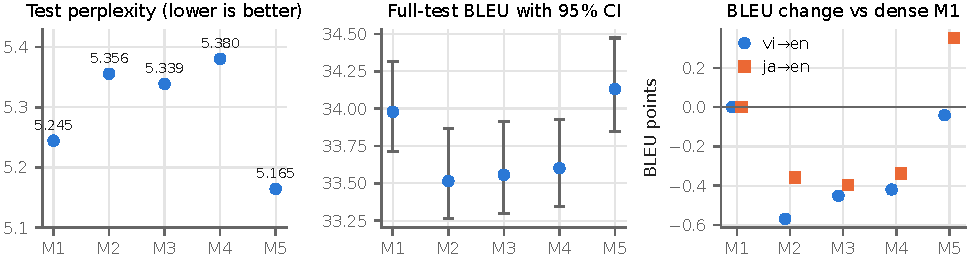
\includegraphics[width=\textwidth]{figures/report/p1_summary.pdf}
\caption{Part 1. Left: test perplexity. Middle: full-test BLEU with bootstrap 95\% CI. Right: BLEU change against the dense model, per source language. The y-axes do not start at zero.}
\label{fig:p1}
\end{figure}

Table~\ref{tab:p1} and Figure~\ref{fig:p1} give the results. Perplexity is computed over a million target tokens and gives a clear order: \textbf{M5 (5.165) $<$ M1 (5.245) $<$ M3 (5.339) $<$ M2 (5.356) $<$ M4 (5.380)}. The same order holds for both source languages.

\textbf{Same total parameters (M2--M4 vs.\ M1).} All three MoE models are slightly worse than the dense model: perplexity is 1.8--2.6\% higher and full-test BLEU 0.38--0.46 lower. They also use 23--35\% fewer parameters per token (17.65--20.80M active vs.\ 27.08M), so when total size is fixed, routing saves compute per token at a small cost in quality. M2, with 35\% fewer active parameters, loses only 2.1\% perplexity. Between the two top-1 models, adding the always-on shared expert (M4) did \emph{not} help here: M4 has more active parameters than M2 but the highest perplexity. Top-2 routing (M3) beats top-1 (M2) in perplexity, in line with its larger active count. The BLEU differences among M2--M4 (33.51--33.60) are far smaller than their CIs.

\textbf{Same active parameters (M5 vs.\ M1).} M5 is the best model on every metric: perplexity falls by 1.5\% (vi 4.451$\to$4.387, ja 6.180$\to$6.080) and BLEU rises from 33.98 to 34.13. Almost all of the BLEU gain is on the harder ja$\to$en direction (+0.35, vs.\ $-0.04$ for vi$\to$en). With the per-token compute held fixed, the 46\% extra (inactive) capacity helps.

\textbf{Significance.} The BLEU gaps are small. On the 1,000-triplet sample, the paired bootstrap differences against M1 are M2 $-0.30$ $[-0.99, 0.45]$, M3 $-0.68$ $[-1.33, 0.15]$, M4 $-0.28$ $[-0.95, 0.52]$ and M5 $+0.24$ $[-0.34, 1.02]$; every interval contains zero. The full-test CIs of M1 and M5 also overlap those of M2--M4. We therefore read the perplexity ordering as the reliable signal and the BLEU ordering as consistent with it but not statistically separated. Removing training-overlap sources (``unseen'') lowers every model's BLEU by about 0.42--0.44 and leaves the ranking unchanged.

\textbf{Other observations.} (i) ja$\to$en is much harder than vi$\to$en for every model (BLEU $\approx$28.4--29.1 vs.\ $\approx$38.5--39.1; perplexity $\approx$6.1--6.3 vs.\ $\approx$4.4--4.6). This is consistent with Japanese differing from English in script and word order (SOV vs.\ SVO), while Vietnamese is SVO and Latin-script. (ii) Validation NLL fell at every one of the 12 evaluations for every model. Validation and test NLL agree within 0.004, so no model overfits in 1.56 epochs; all are still data-limited. (iii) Every model picked the upper pilot LR (grid edge), so a larger one might do better. (iv) The MoE models trained for 17.1--17.6 minutes vs.\ 11.6 for the dense model, despite fewer FLOPs per token. At this scale, gathering tokens into four small expert matrix multiplies is less GPU-efficient than one dense 2048-wide multiply.

\subsection{Expert usage per language and distribution of labour}
\begin{figure}[t]
\centering
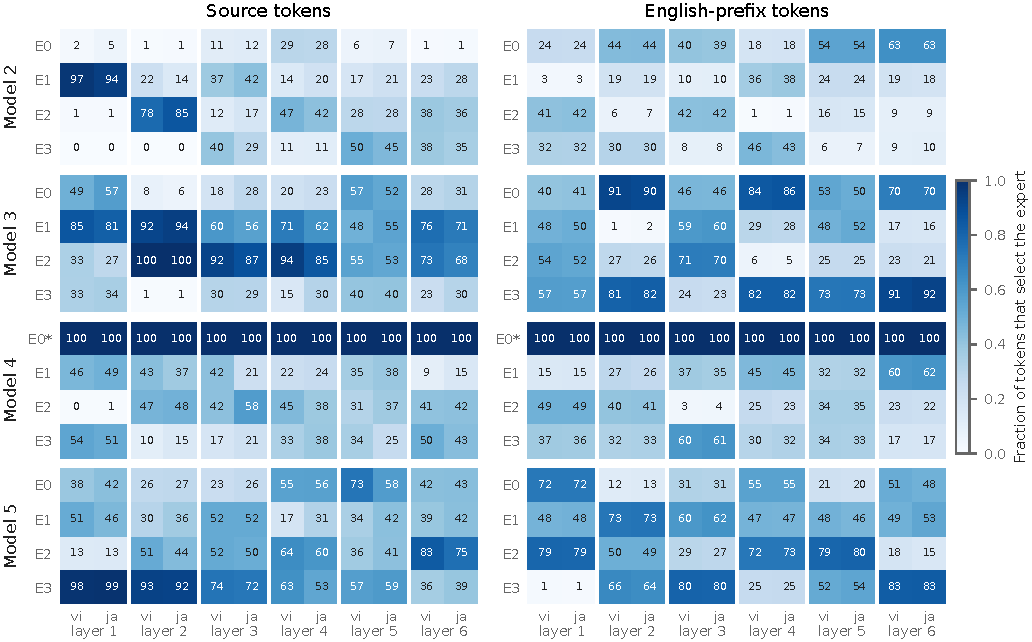
\includegraphics[width=\textwidth]{figures/report/p1_routing.pdf}
\caption{Expert selection rate (\%) per layer, source language and token region, on 1,000 test pairs (about 21k source and 20k English-prefix tokens, teacher forced). For top-2 models a column sums to 200\%. In M4, E0* is the shared expert (100\% by construction).}
\label{fig:routing}
\end{figure}

\begin{table}[t]
\centering\footnotesize
\caption{Routing diagnostics. $H$ is the routing entropy normalised by $\ln(\#\text{routed experts})$ (1 = uniform), shown for layer 1 and averaged over layers and languages. ``Max share'' is the largest fraction of all routed assignments taken by one expert in any layer (the maximum is 0.5 under top-2). ``Unused'' counts (layer, language, region) cells in which some expert is never selected.}
\label{tab:routing}
\begin{tabular}{@{}c ccc ccc c@{}}
\toprule
& \multicolumn{3}{c}{Source tokens} & \multicolumn{3}{c}{English-prefix tokens} & \\
\cmidrule(lr){2-4}\cmidrule(lr){5-7}
M & $H$ layer 1 & mean $H$ & max share & $H$ layer 1 & mean $H$ & max share & Unused\\
\midrule
\rows{tex/p1_routing.tex}
\bottomrule
\end{tabular}
\end{table}

Figure~\ref{fig:routing} shows which experts each language activates; Table~\ref{tab:routing} summarises the balance. Four patterns stand out.

\textbf{1. Routing does not depend on the source language.} In every model and layer, the vi and ja columns are nearly identical. We measured the total-variation distance between the vi and ja routing distributions: at most 0.20 on source tokens (M4, layer 3) and at most 0.03 on English-prefix tokens. Even in layer 1, where Latin-script Vietnamese and Japanese kana/kanji have completely different embeddings, both go to the same expert (M2: E1 takes 97\% of vi and 94\% of ja source tokens). We had expected per-language experts; the models instead learned experts that are shared across languages.

\textbf{2. Experts specialise by token role.} The split is between \emph{source} tokens and \emph{English} tokens. In M2 layer 1, E1 takes 97\% of source tokens but only 3\% of English tokens. In M5 layer 1, E3 is in the top-2 of 98--99\% of source tokens but only 1\% of English tokens. The router learns from the first layer onwards which side of \texttt{[SEP]} a token is on.

\textbf{3. Labour is most uneven in early layers on the source side.} Top-1 routing (M2) nearly collapses there (layer-1 entropy 0.11--0.18; layer 2 sends 78--85\% of source tokens to E2). Deeper layers are much more even (entropy $\approx$0.8--0.9). With top-2 (M3), layer-2 source tokens use a nearly fixed pair (E2 in 99.9\% and E1 in 92--94\% of cases), which behaves like a dense layer. English-prefix tokens are spread more evenly in every model, and M5, whose experts are twice as wide, is the most balanced overall (mean source $H=0.94$). In M4 the shared expert does the common work, and the routed experts are close to uniform on English tokens (layer-5 $H\approx1.00$) but still skewed on source tokens.

\textbf{4. No expert dies.} Every expert receives tokens in every layer, language and region (0 unused cells out of 96), and final load-balancing losses were 1.01--1.08 (1.0 = uniform). The balancing loss works on all tokens of a batch together, so it prevents collapse in aggregate but does not stop experts from specialising by region, which is exactly what we observe.

%======================================================================
\section{Part 2: Optimizers written from scratch}

\subsection{Setup}
\textbf{Task and data.} A causal language model is trained on \texttt{browndw/human-ai-parallel-corpus} (pinned revision, 66,320 documents that are human- and AI-written versions of the same sources). So that parallel versions of one document never sit in different splits, the corpus is split 90/5/5 by \emph{document family} (the \texttt{doc\_id} prefix): 59,688 / 3,312 / 3,320 documents. A new 16,000-token byte-level BPE tokenizer is trained on the training split only (0 unknown tokens in every split). Documents are wrapped in \texttt{<bos>}/\texttt{<eos>}, concatenated and packed into 256-token blocks. One pass over the 153,169 training blocks (39,211,264 prediction tokens) is the ``1$\times$ dataset'' budget.

\textbf{Model and protocol.} The architecture is Part~1's dense model (27,079,680 parameters; $d=512$, 6 layers, 8 heads, FFN 2048, RoPE, tied embeddings, dropout 0.1). For a fair comparison, every optimizer starts from \emph{the same saved initial weights} (hash-checked), sees the blocks in \emph{the same order} (seed 42), and uses batches of $32\times256=8{,}192$ tokens, linear warm-up over 5\% of tokens then cosine decay to $0.1\times$ the peak LR, global gradient clipping at 1.0, decoupled weight decay and FP16 autocast with a gradient scaler. Only the optimizer and its LR change.

\textbf{Evaluation at every $0.1\times$ of the dataset.} \emph{Validation loss}: mean token cross-entropy over all 8,523 validation blocks. \emph{Test BLEU}: for each of the 8,510 test blocks the model sees the first 128 tokens, greedily generates 64 tokens, and sacreBLEU compares them with the true next 64 tokens. As open-ended continuation with one reference, absolute BLEU is low (below 4); it serves to rank optimizers, not to measure translation quality.

\subsection{Optimizers}
All five subclass only \texttt{torch.optim.Optimizer}; no built-in update rule is called. $g$ is the clipped gradient, $\eta$ the scheduled LR and $\lambda$ the weight decay; every rule first applies decoupled decay, $w\leftarrow(1-\eta\lambda)w$.
\begin{itemize}
\item \textbf{AdamW} (baseline; $\beta=(0.9,0.95)$, $\epsilon=10^{-8}$, $\lambda=0.1$): $m\leftarrow\beta_1m+(1-\beta_1)g$, $v\leftarrow\beta_2v+(1-\beta_2)g^2$, $w\leftarrow w-\eta\,\hat m/(\sqrt{\hat v}+\epsilon)$ with bias-corrected $\hat m,\hat v$.
\item \textbf{NAdamW} (variance-reduced AdamW variant; same hyper-parameters): the same moments, but the update uses the Nesterov look-ahead $\tilde m=\beta_1m+(1-\beta_1)g$ (bias-corrected), so the momentum is applied one step early.
\item \textbf{Lion} (memory-efficient; $\beta=(0.9,0.99)$, $\lambda=0.3$): $w\leftarrow w-\eta\,\mathrm{sign}(\beta_1m+(1-\beta_1)g)$, then $m\leftarrow\beta_2m+(1-\beta_2)g$. It keeps one state tensor instead of two (108\,MB instead of 217\,MB here).
\item \textbf{Muon} (matrix-based; momentum 0.95, $\lambda=0.1$): for the 24 weight matrices inside the blocks (18.87M parameters), $m\leftarrow\beta m+g$, $u=\beta m+g$ (Nesterov), $w\leftarrow w-\eta\sqrt{\max(1,r/c)}\;\mathrm{NS}_5(u)$. $\mathrm{NS}_5$ is five Newton--Schulz iterations $X\leftarrow3.4445X-4.7750(XX^\top)X+2.0315(XX^\top)^2X$ on the normalised $u$, which approximately orthogonalise the update (singular values $\to1$). The tied embedding and the LayerNorm vectors (8.21M parameters) use the hand-written AdamW rule with LR $6\cdot10^{-4}$.
\item \textbf{SophiaG} (bonus, Hessian approximation; $\beta=(0.965,0.99)$, $\rho=0.04$): $m\leftarrow\beta_1m+(1-\beta_1)g$. Every 10 steps the diagonal Hessian estimate $h$ is refreshed with the Gauss--Newton--Bartlett estimator: sample labels from the model's own softmax, back-propagate, and set $h\leftarrow\beta_2h+(1-\beta_2)\hat g^2$. The update is $w\leftarrow w-\eta\,\mathrm{sign}(m)\min(|m|/(\rho Bh+\epsilon),1)$, with $B=8192$.
\end{itemize}
Unit tests check AdamW, NAdamW and Lion against scalar re-implementations of these equations, Muon's step against Nesterov momentum + Newton--Schulz + shape scaling, Newton--Schulz against the exact polar factor from an SVD, and Sophia's clipped ratio against a hand computation.

\subsection{Learning-rate sweep (bonus)}
Each optimizer's peak LR was tuned with proxy runs on $0.1\times$ the data (3,920,896 tokens), each with its own complete warm-up and cosine schedule, from the shared initial weights. The grid was multipliers $\{\tfrac14,\tfrac12,1,2,4\}$ of a base LR (AdamW/NAdamW $6\cdot10^{-4}$, Lion $10^{-4}$, Muon $0.02$, Sophia $3\cdot10^{-4}$), extended by $2\times$ whenever the best value lay on an edge. Selection used validation loss only; the test set was never used. NAdamW and Lion each needed one extension, to $8\times$. Every curve in Figure~\ref{fig:p2}(right) is U-shaped with its minimum inside the grid. \textbf{Muon} is the least sensitive: 5.09--5.33 over a $16\times$ LR range, and below every other optimizer's best value at every LR it tried. \textbf{Lion} is the most sensitive: 6.93 at $\tfrac14\times$ down to 5.86 at $4\times$. \textbf{Sophia} degrades quickly above its base LR (6.32 at $4\times$).

\subsection{Results}
\begin{figure}[t]
\centering
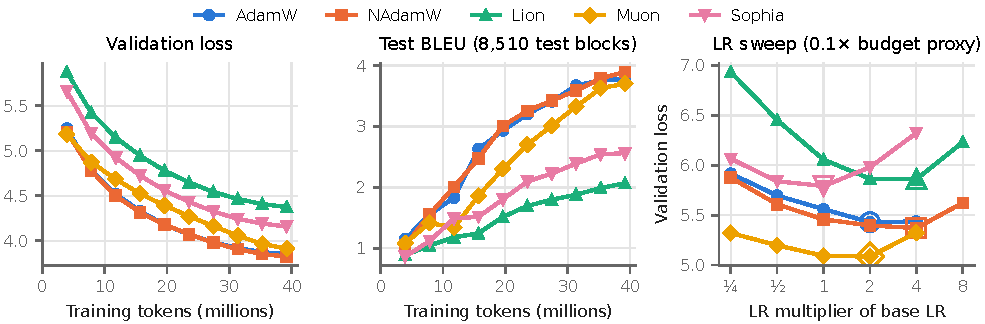
\includegraphics[width=\textwidth]{figures/report/p2_curves.pdf}
\caption{Part 2. Validation loss (left) and test BLEU (middle) at every $0.1\times$ of the dataset; learning-rate sweep on the proxy budget (right, large hollow markers = selected LR).}
\label{fig:p2}
\end{figure}

\begin{table}[t]
\centering\footnotesize\setlength{\tabcolsep}{4pt}
\caption{Part 2 at half and full budget. Wall clock is optimisation time only (excluding evaluation). Peak memory includes evaluation. AMP skips are steps skipped by the FP16 gradient scaler.}
\label{tab:p2}
\begin{tabular}{@{}l c cc c cc c c c@{}}
\toprule
& Selected LR & \multicolumn{2}{c}{Val.\ loss} & Val.\ PPL & \multicolumn{2}{c}{Test BLEU} & Train time & Peak mem. & AMP\\
\cmidrule(lr){3-4}\cmidrule(lr){6-7}
Optimizer & (multiplier) & $0.5\times$ & $1.0\times$ & $1.0\times$ & $0.5\times$ & $1.0\times$ & (s) & (GiB) & skips\\
\midrule
\rows{tex/p2_main.tex}
\bottomrule
\end{tabular}
\end{table}

Figure~\ref{fig:p2} and Table~\ref{tab:p2} give the results. At the full budget the order is \textbf{NAdamW $<$ AdamW $<$ Muon $<$ Sophia $<$ Lion} in validation loss, and exactly the reverse in test BLEU. BLEU rises with training for every optimizer (Muon has a single dip, at $0.3\times$) and tracks validation loss closely, which suggests continuation BLEU is a usable, if coarse, proxy here.

\textbf{AdamW vs.\ NAdamW.} The two curves almost overlap. NAdamW ends slightly ahead (3.824 vs.\ 3.849; BLEU 3.89 vs.\ 3.78) with twice the LR ($2.4\cdot10^{-3}$ vs.\ $1.2\cdot10^{-3}$). This fits the Nesterov look-ahead tolerating a larger step. With a single seed, a 0.025-nat gap is too small to call a real difference.

\textbf{Muon} is the fastest optimizer at the start: it has the lowest loss at $0.1\times$ (5.184 vs.\ 5.209 NAdamW and 5.247 AdamW) and the best proxy losses in the sweep. From $0.2\times$ onwards, however, the Adam-family optimizers overtake it and stay ahead (3.913 vs.\ 3.849 at the end). This matches the observation of Wen et al.\ (2025, arXiv:2509.02046) that early-training comparisons can mislead because rankings change as the LR decays. Two likely reasons for Muon's weaker finish are specific to our setup. First, 30\% of the parameters, including the large tied embedding/LM head, use the fallback AdamW with an LR ($6\cdot10^{-4}$) that was not swept and is half of AdamW's tuned LR. Second, our budget is only about 1.4 tokens per parameter. Muon also costs the most time: 631\,s vs.\ 370\,s for AdamW (+70\%), because of the five FP32 Newton--Schulz iterations per matrix per step.

\textbf{Lion} is the weakest, partly because of the sweep. Extra full-budget runs outside the sweep protocol (same initial weights and data order) reached 4.297 at LR $10^{-4}$ and 4.256 at $2\cdot10^{-4}$, both better than 4.374 at the selected $4\cdot10^{-4}$ (BLEU 2.33 and 2.43 vs.\ 2.07). The proxy compresses the whole schedule into 10\% of the steps, which rewards aggressive LRs. Lion's sign update gives every coordinate the same step size, so it is hit hardest when the LR is too high. Even at its best LR, Lion stays behind Sophia. Its memory saving is real but small in practice: peak memory is 4.59 vs.\ 4.69\,GiB, because activations dominate at this model size.

\textbf{Sophia} lands between Muon and Lion. Its logged statistics explain why: 93.0--94.2\% of coordinates hit the clip $\min(\cdot,1)$ throughout training, so the update is mostly $\eta\,\mathrm{sign}(m)$, close to signed momentum like Lion, and curvature only rescales about 6\% of coordinates. A larger $\rho$ would let the Hessian matter more but was not tuned. The Hessian refresh adds an extra backward pass every 10 steps: training takes 12\% longer than AdamW (414\,s) and Sophia has the highest peak memory (4.92\,GiB).

%======================================================================
\section{Part 3: Decoding strategies}

\subsection{Setup and implementation}
\textbf{Model and data.} \texttt{EleutherAI/pythia-160m} (pinned, FP32) on the whole ROCStories test split (\texttt{hamishivi/ROCStories}, pinned): 19,611 stories, after excluding 22 rows whose reference continuation is empty. The prompt is the story's first sentence; the reference is the remaining four sentences (mean 42.2 Pythia tokens). Each strategy generates at most 64 tokens and stops at EOS. Newline tokens (188 ids) are banned for every strategy because a story is a single paragraph.

\textbf{Decoding from \texttt{model.forward()}.} \texttt{generate()} is never used (the experiment sets it to \texttt{None}). Prompts are left-padded with explicit position ids, and every step feeds one new token per row through the model with a KV cache.
\begin{itemize}
\item \textbf{Greedy}: argmax of the masked logits.
\item \textbf{Beam search} (width $k$): each prompt's cache is copied $k$ times, and every beam except the first starts at $-\infty$. At each step, the $2k$ best of the $k\cdot V$ extensions are ranked by cumulative log-probability. An EOS extension ranked in the top $k$ becomes a finished hypothesis; the others fill the $k$ live beams, and the cache is reordered to match. A prompt finishes once it has $k$ finished hypotheses. The winner maximises $\text{score}/\text{length}^{\alpha}$ with $\alpha=1$.
\item \textbf{Top-$k$}: logits below the $k$-th largest are set to $-\infty$. \textbf{Top-$p$}: the smallest set of tokens, in descending order, whose mass reaches $p$, including the token that crosses $p$, so the most likely token is always kept. \textbf{Pure sampling}: the full softmax at temperature 1.
\end{itemize}
Sampling runs use seeds 0, 1, 2. Unit tests check that cached left-padded decoding equals uncached decoding, that beam-1, top-$k{=}1$ and top-$p{\to}0$ equal greedy, that exhaustive beam search finds the most probable sequence, and that beam results do not depend on batching.

\textbf{Metrics} (per story, then averaged). \emph{Perplexity}: $\exp(\sum\text{NLL}/\#\text{tokens})$ of a strategy's own output (including EOS) under the unmodified model. The human reference continuations score \textbf{24.71}. \emph{Accuracy}: position-by-position match between generated and reference Pythia tokens, divided by the reference length. \emph{Precision/recall/F1}: overlap between the multisets of lower-cased, punctuation-free words of the generation and of the reference. We also record corpus-level distinct-$n$, the fraction of trigrams that repeat earlier in the same text, and the fraction of outputs ending in EOS.

\subsection{Results}
\begin{table}[t]
\centering\footnotesize\setlength{\tabcolsep}{3.3pt}
\caption{Part 3 on 19,611 ROCStories test stories; sampled rows are means over 3 seeds ($\pm$ std; std $\le0.0015$ elsewhere). Gen.\ PPL: model perplexity of its own output (human reference 24.71). Rep-3: repeated-trigram fraction. Len: mean tokens. Stop: fraction ending in EOS. Time: full-run decode seconds (batch 128 greedy/sampling, 32 beam).}
\label{tab:p3}
\begin{tabular}{@{}l c ccc c c cc cc r@{}}
\toprule
Strategy & Accuracy & Prec. & Recall & F1 & Gen.\ PPL & Distinct-2 & Rep-3 & Len & Stop & Time (s)\\
\midrule
\rows{tex/p3_main.tex}
\bottomrule
\end{tabular}
\end{table}

\begin{figure}[t]
\centering
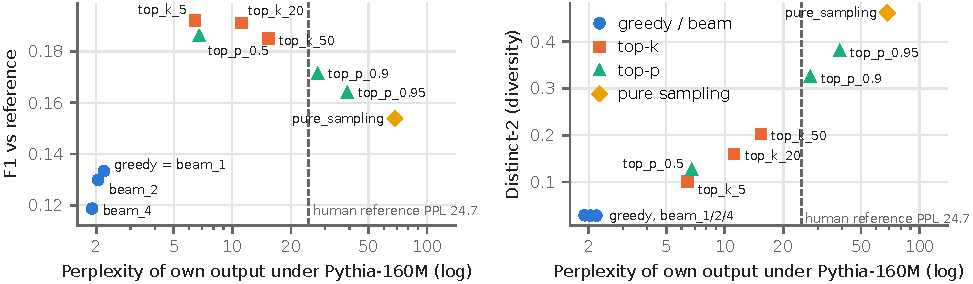
\includegraphics[width=\textwidth]{figures/report/p3_quality_diversity.pdf}
\caption{Each strategy's F1 against the reference (left) and diversity (distinct-2, right), plotted against the perplexity of its own outputs (log scale). The dashed line marks the human reference perplexity (24.71).}
\label{fig:p3}
\end{figure}

\begin{table}[t]
\centering\footnotesize
\caption{Story 1 of the test split (verbatim, cut at ``\ldots''). Sampled outputs use seed 0.}
\label{tab:gen}
\begin{tabular}{@{}>{\bfseries}l p{0.83\textwidth}@{}}
\toprule
Prompt & Dave went to Mammoth Mountain to go skiing.\\
Reference & He put on his boots, skis and goggles. With great excitement, he climbed into the chair lift. There was a foot of fresh powder from a recent storm. Dave jumped off the chair lift and took off down the mountain.\\
\midrule
Greedy & He was a good skier, but he was a bit of a skier. He was a good skier, but he was a bit of a skier. He was a good skier, but he was a bit of a skier. He \ldots\\
Beam-4 & The first thing he did was go to the top of the mountain, and then he went back to the top of the mountain. Then he went back to the top of the mountain, and then he went back to \ldots\\
Top-$k$ 50 & His mother said he was great at taking care of his girlfriend, who told him in the last scene that he was born in the park, so he was good at ski jumping, in this scene of the little house \ldots\\
Top-$p$ 0.9 & His grandma did the thing before, and we had things done there too, in the way I went to Canada in 2007. We went for short walks, and put on my gloves. The first day we drove up on March \ldots\\
Pure & His grandma did the thing before, and we had things done there too, in the safe haven of a place known as the Victoria Reservoir. Last semester (other than in this old-school TV house salvage place) \ldots\\
\bottomrule
\end{tabular}
\end{table}

Table~\ref{tab:p3} and Figure~\ref{fig:p3} summarise the metrics, and Table~\ref{tab:gen} shows one story.

\textbf{Deterministic decoding degenerates.} Greedy and beam outputs have very low perplexity (2.19 greedy, 1.90 beam-4) because they loop. 71--74\% of their trigrams repeat earlier ones, and distinct-2 is only 0.028--0.029. In Table~\ref{tab:gen} greedy repeats one sentence and beam-4 a clause; story 0 behaves the same way (``He was a great mentor to me.'' $\times$6). A wider beam finds higher-likelihood text, but that text is \emph{more} repetitive (Rep-3 0.714$\to$0.742) and further from the reference (F1 0.133$\to$0.119). Likelihood and quality diverge here: the most probable continuation under the model is a loop, not a story (the degeneration described by Holtzman et al., 2020). The model also almost never emits EOS (stopped fraction 0.3--4.3\%), so most outputs run the full 64 tokens, about 1.5 times the average reference length.

\textbf{Truncated sampling gives the best content overlap.} Every sampling method has higher precision, recall and F1 than every deterministic one. Top-$k$=5 is best (F1 0.192), followed by top-$k$=20 (0.191). Widening the candidate set ($k$: 5$\to$50, $p$: 0.5$\to$0.95$\to$1) raises diversity monotonically (distinct-2 0.10$\to$0.46) and raises output perplexity from 6.4 to 68.2, while F1 falls steadily. Top-$p$=0.9 (27.5) lands closest to the human perplexity of 24.7, and top-$k$=50 (15.3) is the next closest. In Table~\ref{tab:gen}, top-$k$=50 keeps the skiing topic (``ski jumping''); top-$p$=0.9 and pure sampling drift into unrelated first-person narratives with invented details (``Canada in 2007'', ``Victoria Reservoir''). Top-$p$ 0.9 and pure sampling begin identically because both use seed 0, and hence the same random numbers; seed std is tiny ($\le$0.0007 in F1).

\textbf{Accuracy is near the floor for every strategy} (1.2--2.9\%). Position-wise matching against one human continuation punishes any one-token shift; deterministic decoding ranks first only because high-probability tokens line up with the reference most often. Bag-of-words F1 is the more meaningful overlap metric here, and even it stays below 0.2 because many continuations are valid.

\subsection{Beam-search time and complexity}
\begin{table}[t]
\centering\footnotesize
\caption{Beam timing on a fixed 256-story subset (CUDA-synchronised, after a warm-up). ``Rows'' is the number of sequences per forward call.}
\label{tab:timing}
\begin{tabular}{@{}c ccc cccc@{}}
\toprule
& \multicolumn{3}{c}{1 prompt per batch} & \multicolumn{4}{c}{32 prompts per batch}\\
\cmidrule(lr){2-4}\cmidrule(lr){5-8}
Width $k$ & ms/forward & ms/story & peak MiB & rows & ms/forward & ms/story & peak MiB\\
\midrule
\rows{tex/p3_timing.tex}
\bottomrule
\end{tabular}
\end{table}


\textbf{Complexity.} Let $k$ be the beam width, $T$ the number of generated tokens, $V$ the vocabulary, $C$ the cost of one token through the network, and $L,d$ the number of layers and the model width. Each of the $T$ steps runs one forward pass on $k$ rows, costing $O(k\,(C+L\,d\,t))$ at step $t$ with a KV cache. It then scores $k\cdot V$ extensions with a log-softmax and a top-$2k$ selection ($O(kV)$) and reorders the cache ($O(k\,L\,d\,t)$). In total, beam search costs
\[
O\big(T\,k\,C \;+\; k\,L\,d\,T^2 \;+\; T\,k\,V\big)\ \text{time}, \qquad O\big(k\,L\,d\,(n_{\text{prompt}}+T) + kV\big)\ \text{memory},
\]
which is \emph{linear in $k$}: $k$ times the work of greedy decoding ($k=1$), but with the same number $T$ of sequential steps.

\textbf{Measurements} (Table~\ref{tab:timing}; plot in \texttt{report/figures/part3/beam\_width\_timing.png}). The linear term only shows once the GPU is busy. With one prompt per batch, a forward call costs 10.0--11.1\,ms at every width from 1 to 16: the 160M-parameter model leaves the GPU under-used, so step latency, not FLOPs, sets the time, and 16 beams are almost free. With 32 prompts per batch, the cost per call grows by $1.18\times$, $1.29\times$, $1.70\times$ and $1.92\times$ for each doubling of $k$, approaching the predicted $2\times$ once there are 256--512 rows per call. Memory is exactly linear: each extra beam row costs 6.59\,MiB at every step of the grid. That is of the size expected for one row's KV cache ($2\times12$ layers $\times768\times4$ bytes = 72\,KiB per cached token, over the padded prompt plus up to 64 generated tokens) plus its $V$-wide logit rows. On the full test split, beam widths 1/2/4 took 513/609/791\,s ($1.19\times$, $1.30\times$ per doubling), in line with the subset. Batching matters far more than width: at $k=1$, 32 prompts per batch cut the time per story from 641\,ms to 25.9\,ms.

\textbf{Greedy vs.\ beam-1.} The two are equal in theory (the unit tests confirm it), yet full-run greedy took 132\,s and beam-1 513\,s. This comes entirely from the batch size (128 vs.\ 32): the cost per forward call is the same (13.4 vs.\ 13.1\,ms), but beam-1 needs four times as many calls. Their outputs agree on 19,522 of 19,611 stories. At all 89 first divergences the two competing tokens are the model's top two, with a median log-probability gap of $3.7\cdot10^{-4}$: floating-point near-ties, not a decoder bug.

%======================================================================
\section{Conclusions}
\textbf{MoE:} at equal total parameters, sparse FFNs give up 2--3\% perplexity for 23--35\% fewer active parameters; at equal active parameters, extra experts (M5) give the best model. Routers specialise by token role and depth, not by language, and the balancing loss keeps every expert in use. \textbf{Optimizers:} tuned AdamW/NAdamW are strongest at this budget; Muon leads early but costs 70\% more time; Sophia acts mostly like signed momentum ($\sim$94\% of coordinates clipped); short-budget LR sweeps can mislead (Lion). \textbf{Decoding:} greedy and beam search fall into repetition loops, which widen with the beam; truncated sampling (top-$k$ 5--50, top-$p$ 0.5--0.9) best matches human continuations; beam search is linear in $k$, but on a GPU its wall-clock cost depends mostly on batching.

\noindent\textit{Code:} \texttt{part 1/}, \texttt{src/part2}, \texttt{src/part3}; results and figures in \texttt{report/}. \textit{LLM use:} drafted with Claude from the project's code and results, as the course announcement permits.

\end{document}
